\section{Voronoi Tessellation Generation}\label{des:sec:vor}
The current best model for creating a Voronoi tessellation uses k-means clustering on all the points in a discrete space to the centres. For every point (the plane is seen as a finite number of pixels) in the plane, $p$, it finds the centre, $c_i$, which is the shortest distance from it, i.e. such that $\sqrt{\big(p(x)-c_i(x)\big)^2 + \big(p(y)-c_i(y)\big)^2}$ is minimised. This is suboptimal as the time taken to create the tessellation relies on the dimensions of the plane and the number of centres therein. Instead we seek a method which is invariant of the plane size and relies solely on the centres. For the sake of decreasing the computation time, this method must also be parallelisable. 
\\
\\
To satisfy these constraints, the divide and conquer algorithm (Section \ref{tes:ssec:dac}) was chosen. The algorithm works by ordering the centres lexicographically and dividing the centres into two subsets, left, $C_L$, and right, $C_R$. The Voronoi tessellations are generated for the left and right subsets separately using the divide and conquer method. The convex hulls of the left and right Voronoi tessellations are then found. The lowest common support line between the hulls is calculated and from this a dividing polygonal chain is generated until it intercepts the upper bounds of the plane. The intersecting edges with the polygonal chain are determined, and lines in the polygonal chain are cut to become part of the Voronoi cells edges.
\\
\\
Code for the Divide and Conquer algorithm was adapted from that in the git repository pyVoronoi\footnote{https://github.com/twmht/pyVoronoi}. pyVoronoi is an implementation for the Divide and Conquer Voronoi algorithm written in Python 2.7. It uses a simple GUI to generate a Voronoi tessellation in a fixed plane using sources read in from a text file. This interface, while simple to use, is constraining as it does not allow users to specify their own spacial constraints or generate the Voronoi as part of a pipelined process. The visualiser and interface were therefore removed and the remaining code re-factored so that the process is a function that can be called by the user or used in a larger process.

\subsection{Structures Used by the Voronoi}\label{sec:des:struct}
The Voronoi structure consists of two main structures, lines and centres. Centres (Section \ref{sec:design:source}) are mainly used to define the sources, but are also used to generate lines.
\\
\\
A line is made up of the following attributes:
\begin{enumerate}
\item Two points, defined as centres which make up the end points of the line. These are defined when the line is created.
\item Two centres which the line bisects, which is set to be empty by default.
\item A centre defining the circumcentre of the line which is empty when the line is created.
\item A list of all lines connected to this one which is used during the merge of the divide and conquer and is empty by default.
\item A Boolean value determining whether the line is active or deprecated. This is set to true by default, but this is updated when two cells are no longer neighbours, generally due to a merge.
\end{enumerate}

\subsection{Voronoi Function}
The Voronoi function takes in the set of centres and a range of centres it will operate on (initially the entire set, $C$). Depending on the number of points in the subset range, one of three operations occurs.
\\
\\
If the range is made up of more than three points, the range is divided into two equal subranges: one from the starting point of the range to the median, $C_L = \{0,...,\frac{n}{2}\}$ where $n$ is the range, and another from the point after the median to the end of the range,$C_R = \{\frac{n}{2}+1,...,n\}$. The Voronoi function is called again for each subrange, denoted as $C_L$ and $C_R$ for left and right subranges respectively, with the full set of points. Once the Voronoi structure for these two have been calculated, the merge function is called with $V_L$ and $V_R$, the Voronoi structures of $C_l$ and $C_R$ respectively, and the function ends as it is not value returning.
\\
\\
If the range is three, the function generates three bisecting lines, $b_{1,2}$, $b_{1,3}$ and $b_{2,3}$ one for each pair of the three points, $c_1$, $c_2$ and $c_3$. The intercept of $b_{1,2}$ and $b_{1,3}$ is determined. If it does not exist, the centres are collinear and an invalid line exists, and the line, $l_{1,3}$ is removed as, lexicographically, $c_2$ must lie between $c_1$ and $c_3$ and $l_{1,3}$ must therefore lie in the cell of $c_2$. If the intercept does exist, it lies on the circumcentre, $cc$, of the triangle formed by the centres and the lines $l_{1,2}$, $l_{1,3}$ and $l_{2,3}$ with the centres as endpoints. The lines, $l_{1,2}$, $l_{1,3}$ and $l_{2,3}$, are ordered by the square of their lengths and the triangle they form is determined as either acute, obtuse or right-angled. The centres and corresponding lines are appended to each centre's list of related centres, e.g. $(c_2,b_{1,2})$ and $(c_3,b_{1,3})$ are appended to $c_1$'s list of related centres. The bisecting lines, $b_{1,2}$, $b_{1,3}$ and $b_{2,3}$, are clipped so that they all intercept at $cc$. Figure \ref{fig:vor_triangle} illustrates this process.
\begin{figure}[H]
\centering
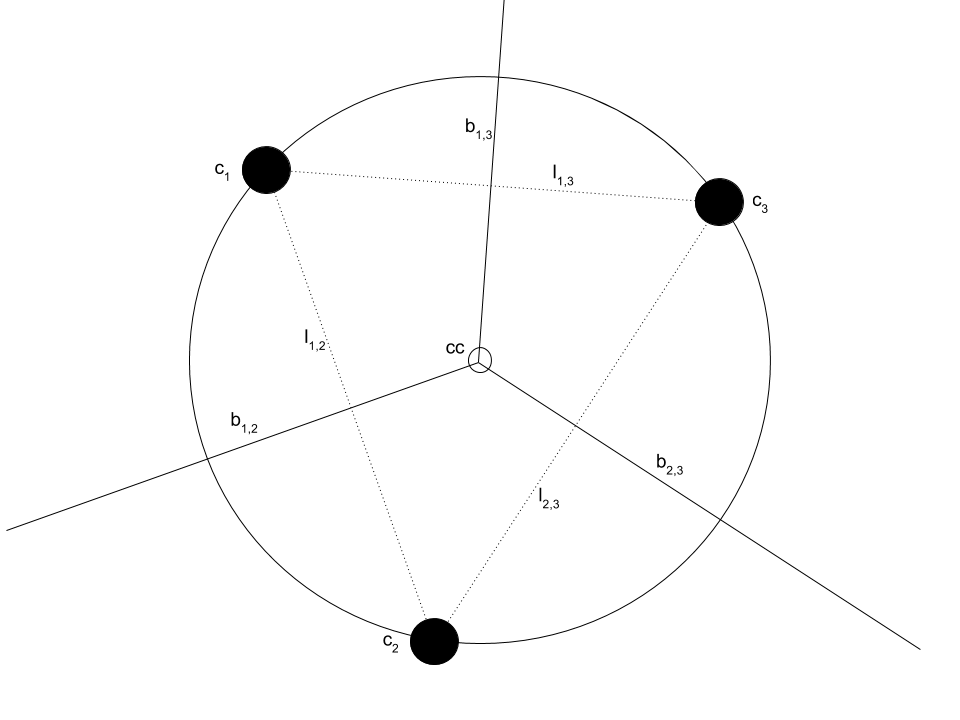
\includegraphics[width=0.8\textwidth]{Images/vor_triangle.png}
\caption{A Voronoi tessellation of three points ($c_1$, $c_2$ and $c_3$) with circumcentre ($cc$).}
\label{fig:vor_triangle}
\end{figure}
A list of the bisecting lines, the range of the points and the convex hull (which is yet to be determined) are returned.
\\
\\
For a range of two points, the bisecting line, $b_{1,2}$, is determined as the only line in the structure. The centres and $b_{1,2}$ are placed into one another's related centre list and the line is placed in a list as the only element. The line list, the range of the centres and their convex hull are returned.
\\
\\
The case of a single centre is excluded as the case of multiple centres divides the set of centres either into two equal subsets or two subsets differing in size by one. The second and third cases will catch sets of three or two centres and therefore the case of a single centre cannot be determined unless a set of a single is passed through initially. This is, however, meaningless as the Voronoi tessellation for this will be a single cell containing the entire space.

\subsection{Convex Hull}
The convex hull of a set of $n$ points, $P = {p_0,p_1,...,p_n}$, is defined as the smallest convex set that contains all the points of $P$. The convex set can be seen as a polygon where each vertex of the polygon is convex (has an internal angle less than $\pi$ radians). For the convex set to be minimal, the vertices of the convex set must lie on a subset of the points of $P$. A convex hull of $P$ can be determined in $O(n\log(n))$ time \citep{eddy1977new}. Figure \ref{fig:convexhull} shows an example of a convex hull.
\begin{figure}[H]
\centering
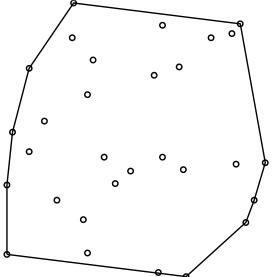
\includegraphics[width=0.5\textwidth]{Images/convexhull.png}
\caption[]{A convex hull of a set of points\footnotemark.}
\label{fig:convexhull}
\end{figure}
\footnotetext{Taken from \url{http://www.evanjones.ca/convexhulls.html}}
Andrew's monotone chain convex hull algorithm \citep{andrew1979another} was used to determine the convex hull of each subset of centres. The function is first passed a range of centres on which to operate. The centres must be ordered lexicographically, which was done before the Voronoi creation process was started. A list of zeros, twice the size of the number of centres in the range is created; this list holds the elements of the chain. The complete convex hull is calculated in two steps, with the first finding the upper hull and the second finding the lower hull.
\\
\\
The first centre, $c_0$, which is also the leftmost centre and the second centre in the range, $c_1$, are both added to the list. The rest of the range is iterated over , adding the next centre to our list, if the angle created by the three points at the end of the list $c_{j-1}$, $c_j$ and $c_{j+1}$, is less than $\pi$ radians. The three centres remain in the list and the next centre, $c_{j+2}$ is added. If the angle is greater than $\pi$ radians, the two centres at the end of the list, $c_j$ and $c_{j+1}$, are removed and the process continues by adding the next point, $c_{j+2}$. This continues until the rightmost centre, $c_n$, is reached, at which time the upper hull of the convex hull has been created.
\\
\\
To generate the lower hull, the same process is used, but the range is iterated over in reverse, starting at the rightmost centre, $c_n$, and ending at the leftmost, $c_0$.
\begin{figure}[H]
\centering
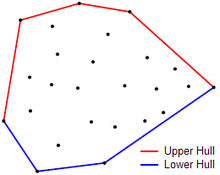
\includegraphics[width=0.5\textwidth]{Images/andrewmonotone.png}
\caption[]{A convex hull created using Andrew's monotone convex hull algorithm with the upper hull in red and the lower hull in blue\footnotemark.}
\label{fig:andrewmonotone}
\end{figure}
\footnotetext{Taken from \url{https://en.wikibooks.org/wiki/Algorithm_Implementation/Geometry/Convex_hull/Monotone_chain}}
Once the list has been populated with the centres of the lower and upper hulls, the monotone chain is formed. The chain is iterated over with each centre in the chain adding the preceding centre to its counter-clockwise parameter and the next point to its clockwise one.

\subsection{Voronoi Merge Function}
The merge begins by finding the upper and lower tangents, $t_u$ and $t_l$ respectively, of the sets $C_L$ and $C_R$. These tangent lines are defined as connections between the convex hulls of $C_L$ and $C_R$ such that they form part of the convex hull of the union of $C_L$ and $C_R$. Starting from the rightmost centre in $C_L$ and the leftmost centre in $C_R$, the algorithm finds the upper tangent by creating two sets of three centres, $(c^L_i,c^L_{i-1},c^R_j)$ and $(c^L_i,c^R_j,C^R_{j+1})$ where $c^L$ and $c^R$ indicate centres in $C_L$ and $C_R$, respectively. These overlapping sets must both satisfy the convex condition, i.e. the angle between these three centres must be less than $\pi$ radians. Once these conditions are met, $t_u$ is created between $C^L_i$ and $C^R_j$. The operation moves counter-clockwise on $C_L$ and clockwise on $C_R$. To find the lower tangent, $t_l$, the order is reversed with $C_L$ stepping clockwise and $C_R$ counter-clockwise. An example of this can be seen in Figure \ref{fig:v_merge1}.
\begin{figure}[H]
\centering
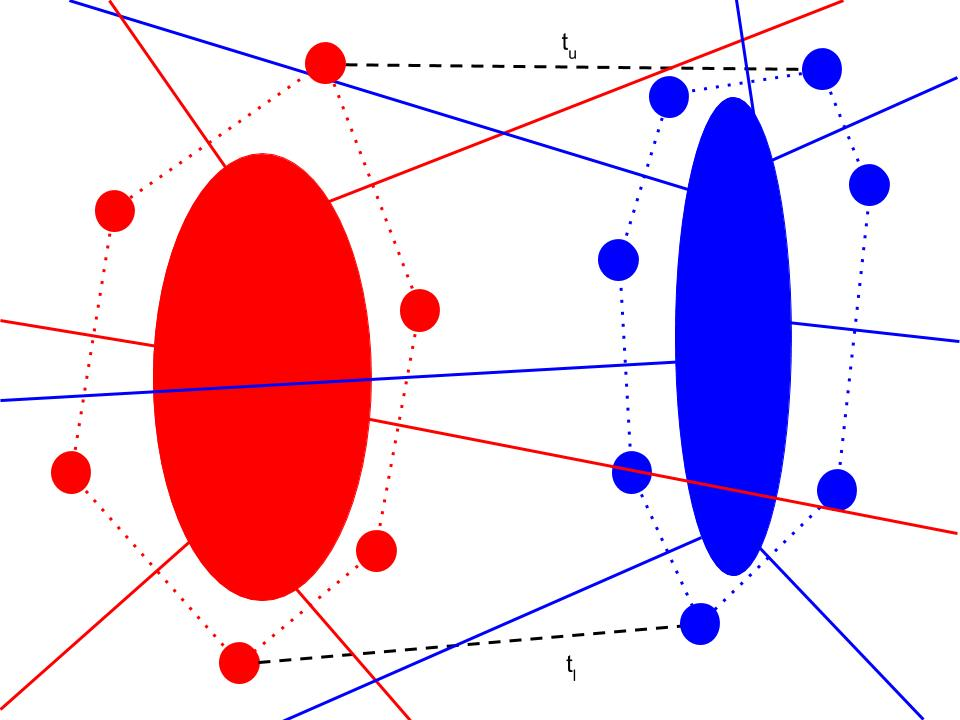
\includegraphics[width=0.6\textwidth]{Images/v_merge1.jpg}
\caption{Two neighbouring tessellations, $C_L$(red) and $C_R$(blue). Only centres affected by the merge on the convex hull and their bisecting lines are shown. The upper and lower tangents, $t_u$ and $t_l$ are shown in black.}
\label{fig:v_merge1}
\end{figure}
The upper tangent, $t_u$, is used to find the starting point of the polygonal chain used to merge the Voronoi. We start by creating an empty list, $HP$, which stores the line segments of the polygonal chain. The bisector of $t_u$, $b_0$, is used as the first line segment in the polygonal chain and is appended to HP. The endpoint of $t_u$ with the greatest $y$ value is determined, $c^u_0$, and a new tangent is generated with the lower centre, $c^u_1$, and a neighbour of $c^u_0$ in the same subset as $c^u_0$, not necessarily in the convex hull, so long as the related line to $c^u_0$ is both available and intercepts $b_0$. The bisecting line of $c^u_0$ and its chosen neighbour is appended to a list of lines which intercepts the polygonal chain, known as \textit{clip\_lines}. The bisector of $c^u_1$ and the chosen neighbour of $c^u_0$ is determined and appended to $HP$ and the process begins anew. An illustration of a step in the process can be seen in the transition from Figure \ref{fig:v_merge2} to Figure \ref{fig:v_merge3}.
\begin{figure}[H]
\centering
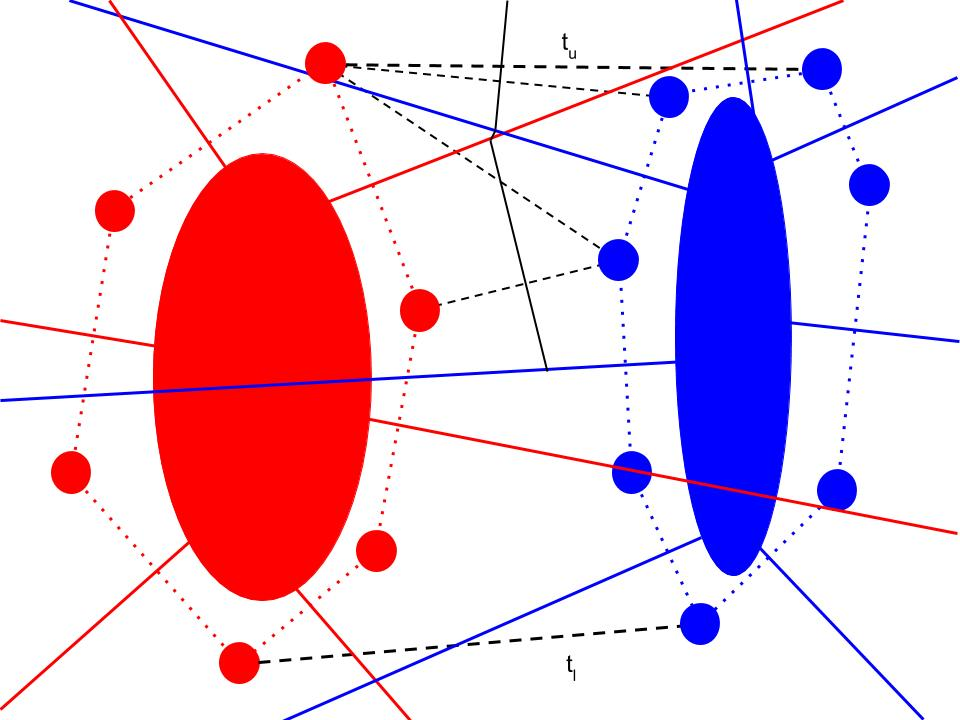
\includegraphics[width=0.6\textwidth]{Images/v_merge2.jpg}
\caption{Two neighbouring Voronoi tessellations merging: the dashed black lines depicting the tangent lines and the solid black line segments depict the growing polygonal chain.}
\label{fig:v_merge2}
\end{figure}
\begin{figure}[H]
\centering
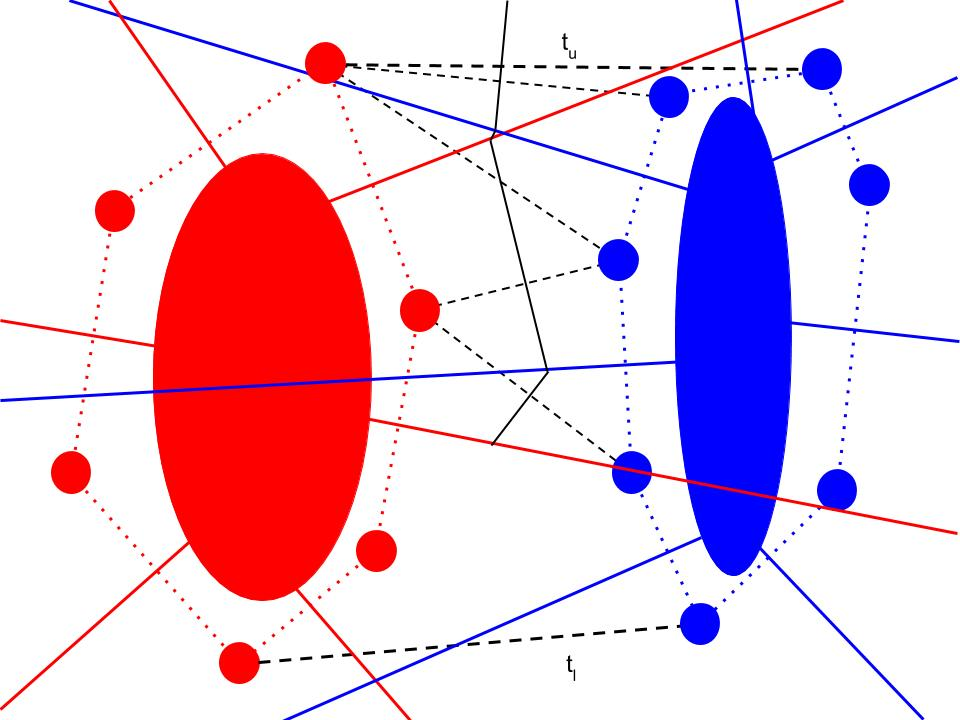
\includegraphics[width=0.6\textwidth]{Images/v_merge3.jpg}
\caption{Two neighbouring Voronoi tessellations continuing to merge.}
\label{fig:v_merge3}
\end{figure}
This process is repeated until the bisecting line of $t_l$ is determined,as shown in Figure \ref{fig:v_merge4}.
\begin{figure}[H]
\centering
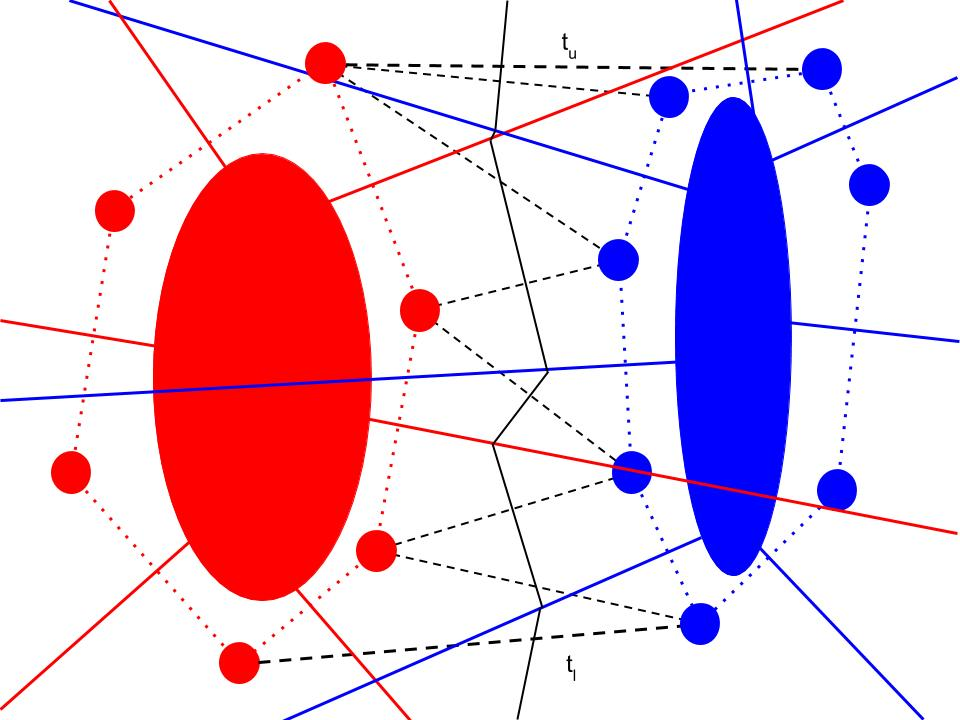
\includegraphics[width=0.6\textwidth]{Images/v_merge4.jpg}
\caption{A near complete Voronoi merge: the lower tangent $t_l$ has been reached by the polygonal chain depicted as solid black line segments.}
\label{fig:v_merge4}
\end{figure}
Once complete, we are left with a list, HP, which contains the bisecting lines between points in $C_L$ and $C_R$ and a list of bisecting lines from $C_L$ and $C_R$, \textit{clip\_lines}. The lines in $HP$ and the centres they bisect are added to the related lists of each of the centres they bisect. The lines in \textit{clip\_lines} are cut at their intercepts and all are appended to a list of lines to be passed back along with the range of points and the new convex hull of the combined Voronoi structure. A depiction of the two Voronoi tessellations with clipped lines can be seen in Figure \ref{fig:v_merge5}.
\begin{figure}[H]
\centering
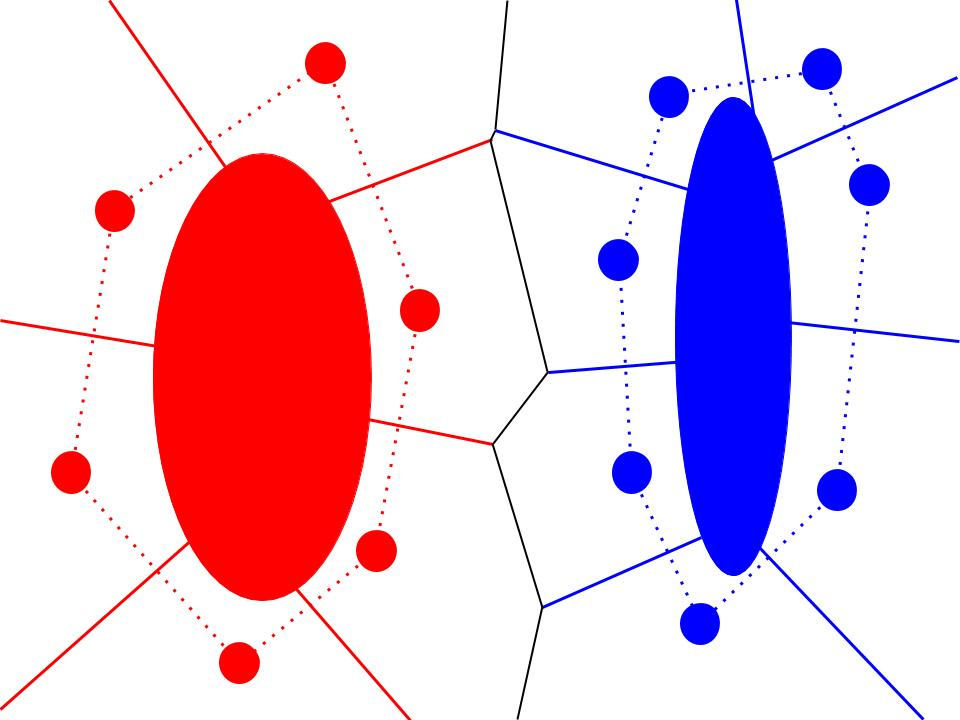
\includegraphics[width=0.6\textwidth]{Images/v_merge5.jpg}
\caption{A completed Voronoi merge, with clipped lines denoting the new cell dimensions.}
\label{fig:v_merge5}
\end{figure}
An example of a complete Voronoi Tessellation is illustrated in Figure \ref{fig:gen_voronoi}.
\begin{figure}[H]
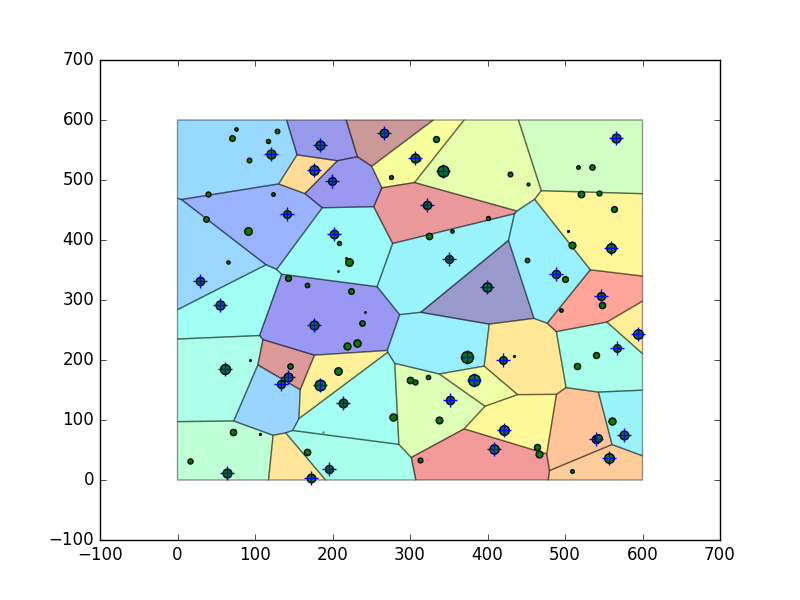
\includegraphics[width=\textwidth]{Images/recentre1.png}
\caption{A Voronoi tessellation generated by the divide and conquer algorithm with sources as circles and stars to represent the Voronoi centres.}
\label{fig:gen_voronoi}
\end{figure}
\subsection{Weighted Voronoi Tessellation}
An attempt was made to generate a weighted Voronoi tessellation using a distance transform which uses the intensities of the centres to redetermine the coordinates of the midpoint of the centres. This transform is defined in Equation (\ref{eq:w_dist}) where $z_1$ and $z_2$, and $\vec{x_1}$ and $\vec{x_2}$ are the intensities and coordinates of $c_1$ and $c_2$, respectively.
\begin{equation}\label{eq:w_dist}
	d'(c_1,c_2) = \frac{z_1}{z_1+z_2}\vec{x_1} + \frac{z_2}{z_1+z_2}\vec{x_2}
\end{equation}
This is an extension of the standard distance equation since, if $z_1=z_2$ we obtain
\begin{align*}
	d'(c_1,c_2) &= \frac{z_1}{z_1+z_2}\vec{x_1} + \frac{z_2}{z_1+z_2}\vec{x_2} \\
	d'(c_1,c_2) &= \frac{1}{2}\vec{x_1} + \frac{1}{2}\vec{x_2} \\ 
	d'(c_1,c_2) &= \frac{\vec{x_1} + \vec{x_2}}{2} \\
\end{align*}
Some complications were found in this during the Voronoi merge process; weighted centres that are not close enough to the convex hull but due to their larger weighting still have cells that dominate areas of the hull were not included in the merging process and their line segments were not clipped or deactivated. Another problem with this is that it generates undefined regions in the space, that is, regions where domains overlap due conflicting weightings, an example of which can be seen in Figure \ref{fig:w_voronoi_issue}.
\begin{figure}[H]
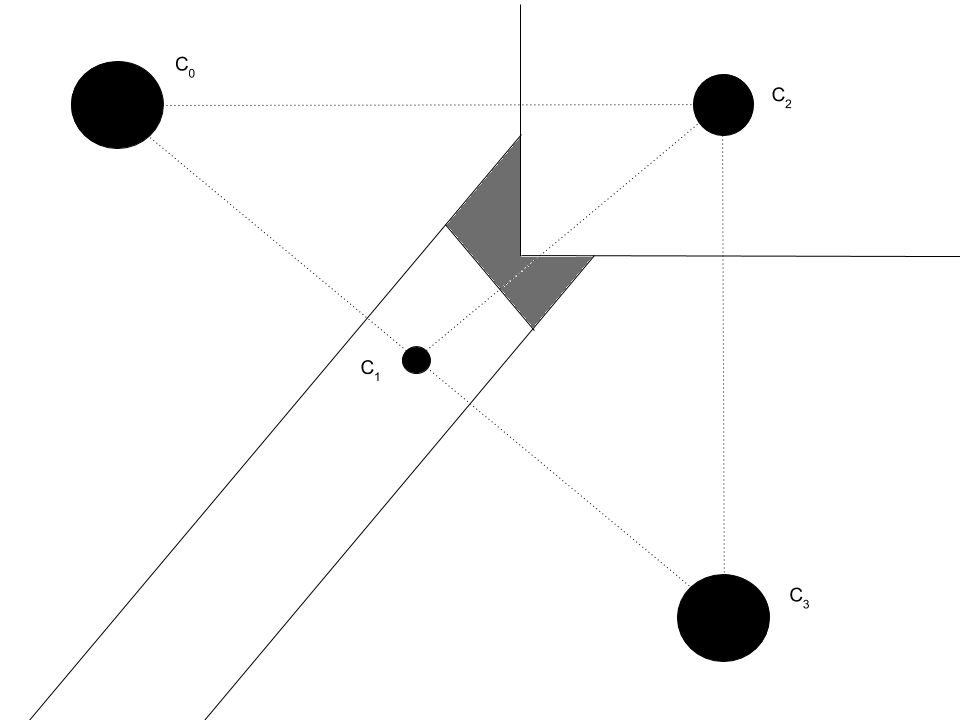
\includegraphics[width=0.5\textwidth]{Images/weighting_problem.png}
\centering
\caption{An unclassified area (grey) generated by a weighting conflict in $c_1$ and $c_2$.}
\label{fig:w_voronoi_issue}
\end{figure}
The figure shows a conflicting area between $c_1$ and $c_2$. It would be expected that $c_2$, with its higher intensity, would claim the area, but in doing so it would cross into the area that should be the domain of $c_0$ or $c_3$. It was for this reason that the choice to use the intensities to weight the Voronoi tessellation creation process was abandoned. Instead the intensities would be used to calculate the error and determine and generate cell merges. An example of a failed weighted Voronoi tessellation can be seen in Figure \ref{fig:w_voronoi}.
\begin{figure}[H]
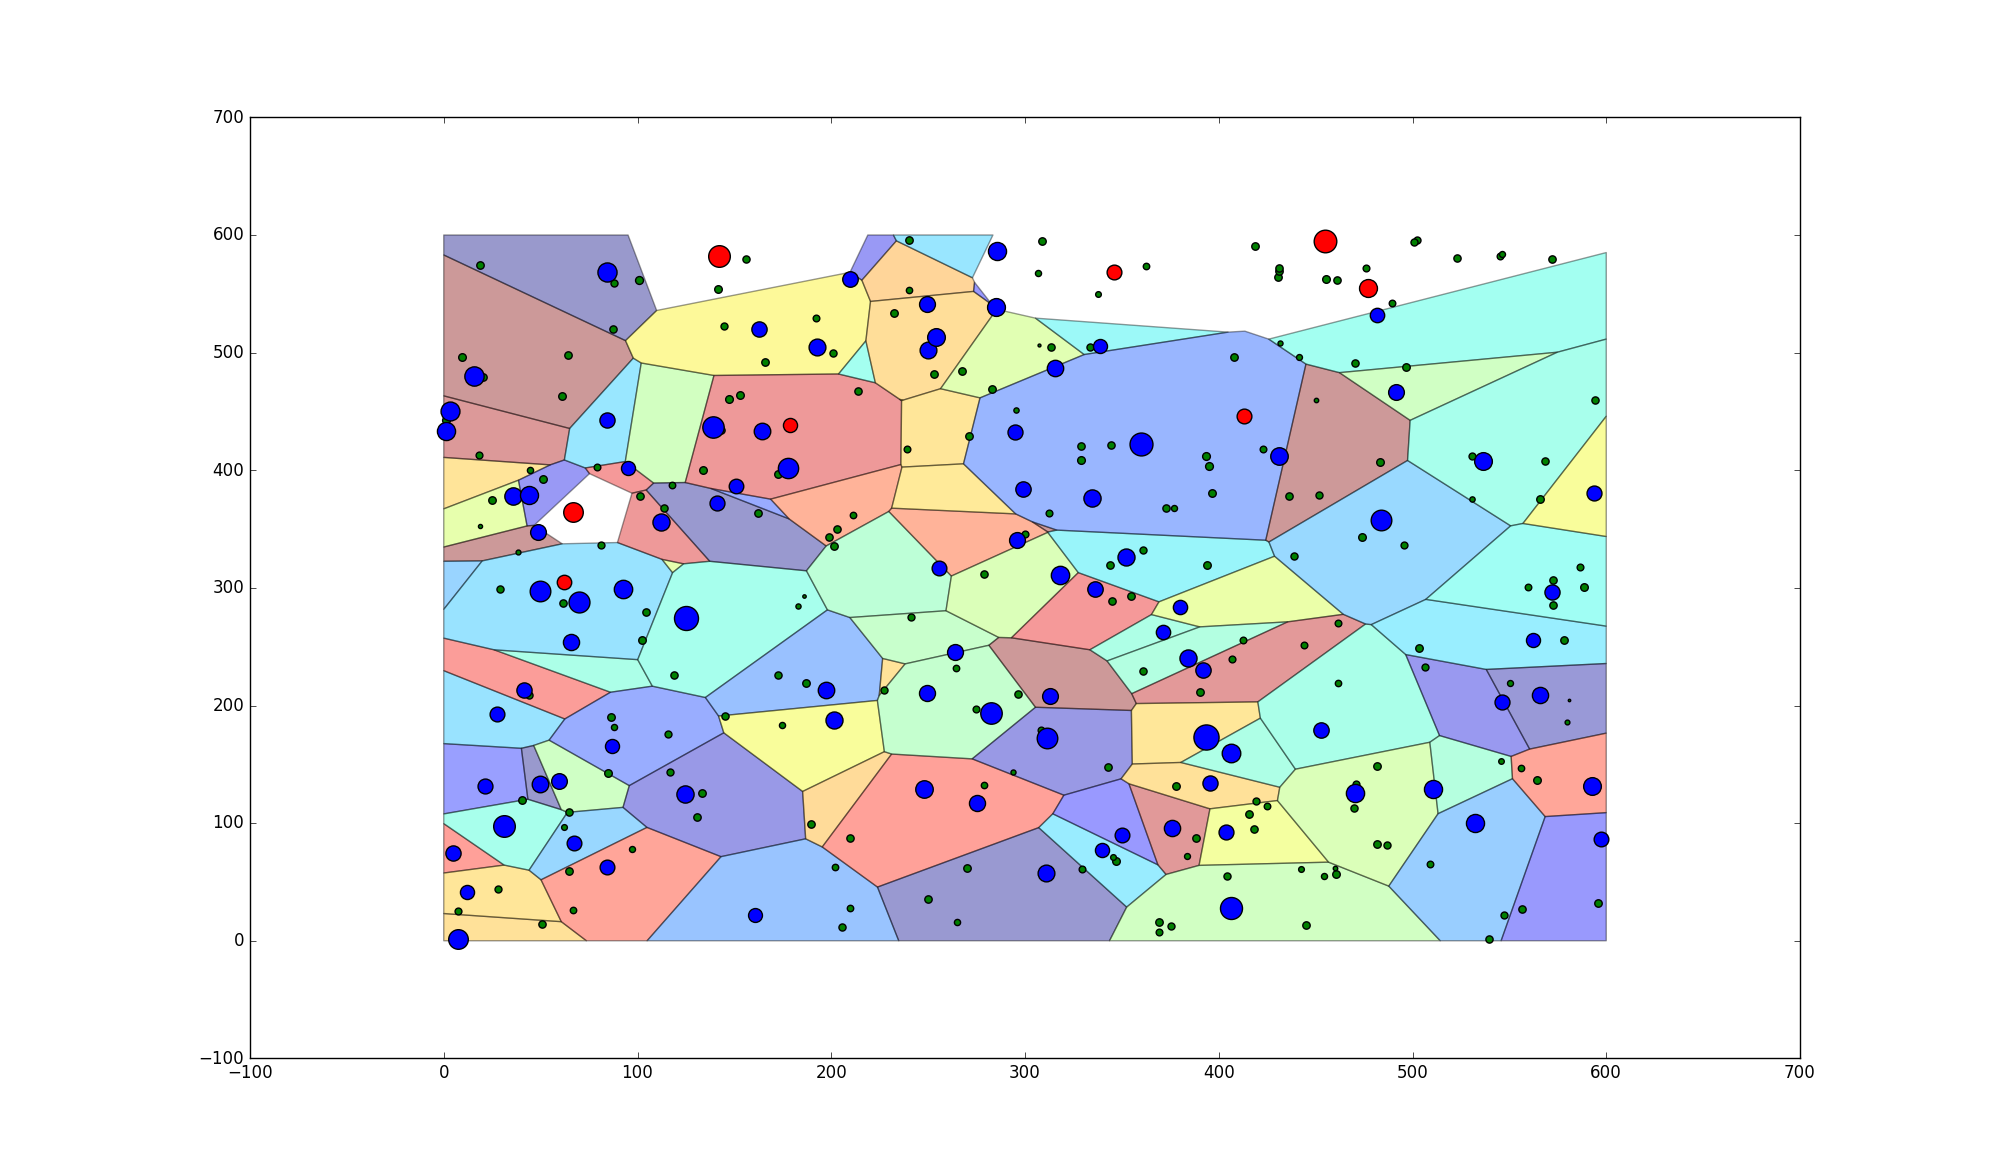
\includegraphics[width=\textwidth]{Images/weighted_voronoi.png}
\centering
\caption{A failed visualisation of a weighted Voronoi tessellation with centres in blue, sources in green and centres without cells in red.}
\label{fig:w_voronoi}
\end{figure}
